% Options for packages loaded elsewhere
% Options for packages loaded elsewhere
\PassOptionsToPackage{unicode}{hyperref}
\PassOptionsToPackage{hyphens}{url}
\PassOptionsToPackage{dvipsnames,svgnames,x11names}{xcolor}
%
\documentclass[
  spanish,
  11pt,
  letterpaper,
]{article}
\usepackage{xcolor}
\usepackage[margin=2.5cm]{geometry}
\usepackage{amsmath,amssymb}
\setcounter{secnumdepth}{5}
\usepackage{iftex}
\ifPDFTeX
  \usepackage[T1]{fontenc}
  \usepackage[utf8]{inputenc}
  \usepackage{textcomp} % provide euro and other symbols
\else % if luatex or xetex
  \usepackage{unicode-math} % this also loads fontspec
  \defaultfontfeatures{Scale=MatchLowercase}
  \defaultfontfeatures[\rmfamily]{Ligatures=TeX,Scale=1}
\fi
\usepackage{lmodern}
\ifPDFTeX\else
  % xetex/luatex font selection
\fi
% Use upquote if available, for straight quotes in verbatim environments
\IfFileExists{upquote.sty}{\usepackage{upquote}}{}
\IfFileExists{microtype.sty}{% use microtype if available
  \usepackage[]{microtype}
  \UseMicrotypeSet[protrusion]{basicmath} % disable protrusion for tt fonts
}{}
\makeatletter
\@ifundefined{KOMAClassName}{% if non-KOMA class
  \IfFileExists{parskip.sty}{%
    \usepackage{parskip}
  }{% else
    \setlength{\parindent}{0pt}
    \setlength{\parskip}{6pt plus 2pt minus 1pt}}
}{% if KOMA class
  \KOMAoptions{parskip=half}}
\makeatother
% Make \paragraph and \subparagraph free-standing
\makeatletter
\ifx\paragraph\undefined\else
  \let\oldparagraph\paragraph
  \renewcommand{\paragraph}{
    \@ifstar
      \xxxParagraphStar
      \xxxParagraphNoStar
  }
  \newcommand{\xxxParagraphStar}[1]{\oldparagraph*{#1}\mbox{}}
  \newcommand{\xxxParagraphNoStar}[1]{\oldparagraph{#1}\mbox{}}
\fi
\ifx\subparagraph\undefined\else
  \let\oldsubparagraph\subparagraph
  \renewcommand{\subparagraph}{
    \@ifstar
      \xxxSubParagraphStar
      \xxxSubParagraphNoStar
  }
  \newcommand{\xxxSubParagraphStar}[1]{\oldsubparagraph*{#1}\mbox{}}
  \newcommand{\xxxSubParagraphNoStar}[1]{\oldsubparagraph{#1}\mbox{}}
\fi
\makeatother


\usepackage{longtable,booktabs,array}
\usepackage{calc} % for calculating minipage widths
% Correct order of tables after \paragraph or \subparagraph
\usepackage{etoolbox}
\makeatletter
\patchcmd\longtable{\par}{\if@noskipsec\mbox{}\fi\par}{}{}
\makeatother
% Allow footnotes in longtable head/foot
\IfFileExists{footnotehyper.sty}{\usepackage{footnotehyper}}{\usepackage{footnote}}
\makesavenoteenv{longtable}
\usepackage{graphicx}
\makeatletter
\newsavebox\pandoc@box
\newcommand*\pandocbounded[1]{% scales image to fit in text height/width
  \sbox\pandoc@box{#1}%
  \Gscale@div\@tempa{\textheight}{\dimexpr\ht\pandoc@box+\dp\pandoc@box\relax}%
  \Gscale@div\@tempb{\linewidth}{\wd\pandoc@box}%
  \ifdim\@tempb\p@<\@tempa\p@\let\@tempa\@tempb\fi% select the smaller of both
  \ifdim\@tempa\p@<\p@\scalebox{\@tempa}{\usebox\pandoc@box}%
  \else\usebox{\pandoc@box}%
  \fi%
}
% Set default figure placement to htbp
\def\fps@figure{htbp}
\makeatother


% definitions for citeproc citations
\NewDocumentCommand\citeproctext{}{}
\NewDocumentCommand\citeproc{mm}{%
  \begingroup\def\citeproctext{#2}\cite{#1}\endgroup}
\makeatletter
 % allow citations to break across lines
 \let\@cite@ofmt\@firstofone
 % avoid brackets around text for \cite:
 \def\@biblabel#1{}
 \def\@cite#1#2{{#1\if@tempswa , #2\fi}}
\makeatother
\newlength{\cslhangindent}
\setlength{\cslhangindent}{1.5em}
\newlength{\csllabelwidth}
\setlength{\csllabelwidth}{3em}
\newenvironment{CSLReferences}[2] % #1 hanging-indent, #2 entry-spacing
 {\begin{list}{}{%
  \setlength{\itemindent}{0pt}
  \setlength{\leftmargin}{0pt}
  \setlength{\parsep}{0pt}
  % turn on hanging indent if param 1 is 1
  \ifodd #1
   \setlength{\leftmargin}{\cslhangindent}
   \setlength{\itemindent}{-1\cslhangindent}
  \fi
  % set entry spacing
  \setlength{\itemsep}{#2\baselineskip}}}
 {\end{list}}
\usepackage{calc}
\newcommand{\CSLBlock}[1]{\hfill\break\parbox[t]{\linewidth}{\strut\ignorespaces#1\strut}}
\newcommand{\CSLLeftMargin}[1]{\parbox[t]{\csllabelwidth}{\strut#1\strut}}
\newcommand{\CSLRightInline}[1]{\parbox[t]{\linewidth - \csllabelwidth}{\strut#1\strut}}
\newcommand{\CSLIndent}[1]{\hspace{\cslhangindent}#1}

\ifLuaTeX
\usepackage[bidi=basic]{babel}
\else
\usepackage[bidi=default]{babel}
\fi
% get rid of language-specific shorthands (see #6817):
\let\LanguageShortHands\languageshorthands
\def\languageshorthands#1{}


\setlength{\emergencystretch}{3em} % prevent overfull lines

\providecommand{\tightlist}{%
  \setlength{\itemsep}{0pt}\setlength{\parskip}{0pt}}



 


\usepackage{booktabs}
\usepackage{longtable}
\usepackage{array}
\usepackage{multirow}
\usepackage{wrapfig}
\usepackage{float}
\usepackage{colortbl}
\usepackage{pdflscape}
\usepackage{tabu}
\usepackage{threeparttable}
\usepackage{threeparttablex}
\usepackage[normalem]{ulem}
\usepackage{makecell}
\usepackage{xcolor}
\usepackage{booktabs}
\usepackage{float}
\makeatletter
\@ifpackageloaded{caption}{}{\usepackage{caption}}
\AtBeginDocument{%
\ifdefined\contentsname
  \renewcommand*\contentsname{Tabla de contenidos}
\else
  \newcommand\contentsname{Tabla de contenidos}
\fi
\ifdefined\listfigurename
  \renewcommand*\listfigurename{Listado de Figuras}
\else
  \newcommand\listfigurename{Listado de Figuras}
\fi
\ifdefined\listtablename
  \renewcommand*\listtablename{Listado de Tablas}
\else
  \newcommand\listtablename{Listado de Tablas}
\fi
\ifdefined\figurename
  \renewcommand*\figurename{Figura}
\else
  \newcommand\figurename{Figura}
\fi
\ifdefined\tablename
  \renewcommand*\tablename{Tabla}
\else
  \newcommand\tablename{Tabla}
\fi
}
\@ifpackageloaded{float}{}{\usepackage{float}}
\floatstyle{ruled}
\@ifundefined{c@chapter}{\newfloat{codelisting}{h}{lop}}{\newfloat{codelisting}{h}{lop}[chapter]}
\floatname{codelisting}{Listado}
\newcommand*\listoflistings{\listof{codelisting}{Listado de Listados}}
\makeatother
\makeatletter
\makeatother
\makeatletter
\@ifpackageloaded{caption}{}{\usepackage{caption}}
\@ifpackageloaded{subcaption}{}{\usepackage{subcaption}}
\makeatother
\usepackage{bookmark}
\IfFileExists{xurl.sty}{\usepackage{xurl}}{} % add URL line breaks if available
\urlstyle{same}
\hypersetup{
  pdftitle={Análisis Bayesiano de la Industria del Anime: Calidad Productiva y Fidelización de Audiencia},
  pdfauthor={Nicolas Sanchez; Adrian Godoy; {[}Nombre{]}; {[}Nombre{]}},
  pdflang={es},
  colorlinks=true,
  linkcolor={NavyBlue},
  filecolor={Maroon},
  citecolor={NavyBlue},
  urlcolor={NavyBlue},
  pdfcreator={LaTeX via pandoc}}


\title{Análisis Bayesiano de la Industria del Anime: Calidad Productiva
y Fidelización de Audiencia}
\usepackage{etoolbox}
\makeatletter
\providecommand{\subtitle}[1]{% add subtitle to \maketitle
  \apptocmd{\@title}{\par {\large #1 \par}}{}{}
}
\makeatother
\subtitle{Propuesta de Proyecto --- Métodos Bayesianos}
\author{Nicolas Sanchez \and Adrian
Godoy \and {[}Nombre{]} \and {[}Nombre{]}}
\date{11 de mayo de 2026}
\begin{document}
\maketitle


\section{Introducción}\label{introducciuxf3n}

La industria del anime constituye uno de los sectores creativos más
sofisticados y de mayor proyección global del entretenimiento
contemporáneo, con una estructura productiva altamente especializada y
una base de audiencia internacional cuyos comportamientos de consumo
presentan características distintivas frente a otras industrias
audiovisuales. Comprender qué factores explican el éxito de un anime
---y, más sutilmente, qué se entiende por ``éxito''--- es una pregunta
de relevancia tanto académica como industrial.

Este proyecto adopta el enfoque de que el éxito de un anime no es un
constructo unidimensional. Específicamente, distinguimos dos dimensiones
empíricamente separables: la calidad evaluativa, expresada como el
promedio de las calificaciones individuales otorgadas por los usuarios,
y la fidelización profunda, expresada como la proporción de usuarios
alcanzados que llegan a establecer un vínculo afectivo identificable con
la obra. Estas dos dimensiones, como mostraremos en el análisis
descriptivo, están correlacionadas pero no son equivalentes: existe una
fracción sustancial de obras donde divergen abiertamente, lo que
justifica estudiarlas como fenómenos distintos y no como dos medidas del
mismo objeto.

A partir de esta distinción, formulamos dos preguntas de investigación
complementarias ---una orientada al lado de la producción, otra al lado
del consumo--- y proponemos abordarlas mediante modelos bayesianos
jerárquicos y de regresión sobre proporciones. La presente propuesta
detalla el contexto del problema, las preguntas centrales, el conjunto
de datos disponible, los criterios de construcción de la muestra de
estudio y los resultados de un análisis descriptivo extensivo orientado
a justificar las decisiones de modelado del informe final.

\section{Contexto y Preguntas de
Investigación}\label{contexto-y-preguntas-de-investigaciuxf3n}

\subsection{Contexto del fenómeno}\label{contexto-del-fenuxf3meno}

La industria del anime ha alcanzado una escala económica y cultural
considerable. De acuerdo con la Asociación de Animación Japonesa (AJA)
(2024-\/-2025), el mercado global del anime ---considerando ventas
internas, licencias internacionales, mercancía derivada y servicios de
distribución digital--- alcanzó un valor de mercado récord de 3,84
billones de yenes (aproximadamente 25 mil millones de dólares
estadounidenses) en 2024, con un crecimiento sostenido impulsado en
buena medida por la expansión de plataformas de streaming
internacionales y por la consolidación de comunidades de fans fuera de
Japón. En este ecosistema, las decisiones de inversión en nuevas
producciones se apoyan en métricas observables tanto sobre la recepción
crítica como sobre la profundidad del compromiso de la audiencia.

En este contexto industrial, dos preguntas de naturaleza distinta
---pero estrechamente relacionadas--- resultan particularmente
relevantes. La primera se sitúa en el lado de la producción: existen
estudios de animación con larga trayectoria que se han especializado en
distintos tipos de obras (adaptaciones de manga, novelas ligeras,
novelas visuales, videojuegos, o producciones originales), y es
razonable preguntarse si esta especialización se traduce en diferencias
sistemáticas en la calidad evaluativa de sus producciones ---es decir,
si existen ``ventajas'' identificables de cierto estudio para cierto
tipo de material. La segunda se sitúa en el lado del consumo: en una
industria donde la popularidad masiva (medida por la audiencia
alcanzada) y la fidelización profunda (medida por la intensidad del
compromiso emocional) son métricas que no necesariamente coinciden,
conviene preguntarse qué géneros narrativos generan mayor identificación
afectiva entre los espectadores que los consumen, una vez controlado el
efecto del simple alcance comercial.

Ambas preguntas comparten una característica metodológica común:
involucran comparaciones entre numerosas categorías (más de 400
estudios, 21 géneros principales) con tamaños muestrales muy desiguales
---desde estudios con cientos de obras hasta géneros de nicho con apenas
decenas de animes. Este desbalance hace que los enfoques estadísticos
clásicos produzcan estimaciones inestables para las categorías menos
representadas, mientras que los métodos bayesianos jerárquicos
---mediante el mecanismo de partial pooling--- permiten combinar
información a través de las categorías de forma estadísticamente
principada, ofreciendo además una cuantificación natural de la
incertidumbre asociada a cada inferencia.

\subsection{Preguntas de
investigación}\label{preguntas-de-investigaciuxf3n}

A partir del contexto descrito, este proyecto se estructura en torno a
dos preguntas de investigación complementarias. La primera adopta una
perspectiva orientada al lado de la producción y se centra en la calidad
evaluativa; la segunda adopta una perspectiva orientada al lado del
consumo y se centra en la fidelización profunda.

\subsubsection{Pregunta 1 --- Lado de la
producción}\label{pregunta-1-lado-de-la-producciuxf3n}

\textbf{¿Existen diferencias sistemáticas en el nivel de calidad típico
---medido a través del Score promedio en MyAnimeList--- entre los
distintos estudios de animación cuando adaptan diferentes tipos de
material original (manga, novela ligera, novela visual, videojuego u
obra original)?}

La industria del anime es un sistema productivo altamente especializado
en el que distintos estudios han desarrollado a lo largo de décadas
capacidades técnicas y estilísticas particulares. Una pregunta central
tanto para inversores como para productores es si esa especialización se
traduce en una ventaja real al adaptar ciertos tipos de obras
originales, o si la calidad del producto final depende principalmente
del propio material de origen y no del estudio responsable.

Investigamos si los estudios presentan diferencias sistemáticas en el
nivel de calidad típico de sus producciones, controlando por el tipo de
material adaptado y por covariables estructurales relevantes. El número
de obras producidas por cada estudio varía drásticamente ---desde unos
pocos títulos hasta varios cientos---, lo que vuelve poco confiables las
estimaciones frecuentistas para estudios con escasa producción. Un
modelo jerárquico bayesiano permite encoger (partial pooling) las
estimaciones de estudios con poca evidencia hacia el promedio global,
distinguiendo así diferencias reales de fluctuaciones por azar y
preservando la individualidad de los estudios con evidencia abundante.

Planeamos abordar esta pregunta mediante un modelo de regresión
jerárquico bayesiano con efectos por estudio sobre el Score, incluyendo
el material original como covariable de interés. La especificación
detallada del modelo se desarrollará en el informe final, sobre la base
de las observaciones empíricas presentadas en el análisis descriptivo.

\subsubsection{Pregunta 2 --- Lado del
consumo}\label{pregunta-2-lado-del-consumo}

\textbf{¿Qué géneros narrativos están asociados a mayor fidelización
profunda ---medida como la proporción Favorites/Members--- entre la
audiencia, una vez controlados el tamaño absoluto del público y los
posibles efectos de acumulación temporal?}

En la industria del entretenimiento, la popularidad masiva (cantidad de
usuarios alcanzados) y la fidelización profunda (intensidad del
compromiso emocional) son dimensiones distintas del éxito. Un anime
puede ser muy visto sin generar identificación fuerte, mientras que otro
puede tener una audiencia reducida pero altamente comprometida
---distinción central para decisiones de mercadotecnia, desarrollo de
mercancía derivada y construcción de comunidades de fans.

Estudiamos qué géneros narrativos están asociados con mayores tasas de
fidelización profunda, definidas como la proporción de usuarios que
marcan un anime como favorito sobre el total de usuarios que lo
registran en su lista. La razón Favorites/Members presenta
sobredispersión sustancial ---pues las decisiones individuales de los
usuarios están correlacionadas dentro de un mismo anime por efectos de
comunidad y recomendación--- y una fracción importante de animes
presenta tasas de fidelización muy bajas o nulas, condiciones que
invalidan un modelo binomial estándar. El enfoque bayesiano permite
incorporar priors débilmente informativos para regularizar los efectos
de géneros altamente correlacionados (un mismo anime suele tener varias
etiquetas simultáneas) y cuantificar directamente la incertidumbre del
ranking de géneros mediante la distribución posterior.

Planeamos abordar esta pregunta mediante un modelo de regresión
bayesiana sobre la proporción de favoritos, capaz de manejar
sobredispersión, controlando por el año de estreno y el tipo de obra. La
especificación detallada se desarrollará en el informe final.

\section{Datos}\label{datos}

\subsection{Procedencia y muestra}\label{procedencia-y-muestra}

Los datos utilizados en este proyecto provienen del sitio MyAnimeList
(MAL) (MyAnimeList LLC 2025), una de las plataformas comunitarias más
grandes del mundo dedicada al seguimiento, calificación y discusión de
obras de anime y manga. MyAnimeList constituye un repositorio
particularmente rico para el análisis cuantitativo del anime: combina
metadatos productivos curados editorialmente (estudio, productor,
material original, fecha de estreno, género) con métricas agregadas de
comportamiento de los usuarios (calificación promedio, número de
usuarios que registran la obra en su lista, número de usuarios que la
marcan como favorita).

El conjunto de datos específico empleado fue publicado en Kaggle bajo el
título \emph{MyAnimeList 2025} (Apriansyah 2025) y corresponde a una
extracción automatizada realizada en noviembre de 2025 sobre el archivo
estacional de MAL (\emph{Season Archive}). El dataset original contiene
\textbf{19.931 registros únicos de anime} y \textbf{25 variables} que
combinan campos de identificación, metadatos productivos, métricas de
audiencia e información estructurada sobre personajes. La cobertura
comprende obras estrenadas desde la década de 1960 hasta el año 2025, en
distintos formatos (TV, película, OVA, ONA, especiales).

Para los objetivos analíticos de este proyecto, se trabaja sobre un
subconjunto cuidadosamente filtrado del dataset original. La
construcción de este subconjunto se detalla en la Sección 3.3, y el
resultado final es una muestra de aproximadamente \textbf{4.500 anime de
tipo TV} sobre la cual se centran ambos modelos del proyecto.

\subsection{Definición de variables}\label{definiciuxf3n-de-variables}

La Tabla 1 resume las variables utilizadas en el análisis, agrupadas
según su rol metodológico. Se incluyen únicamente las variables del
dataset original que efectivamente se emplean en alguno de los dos
modelos o en el análisis descriptivo; campos auxiliares (URL de imagen,
identificador interno de MAL, lista de personajes en formato JSON,
descripción narrativa) se excluyen de esta tabla por no aportar al
análisis estadístico.

\begin{longtable}[t]{>{\raggedright\arraybackslash}p{2.2cm}>{\raggedright\arraybackslash}p{2.8cm}>{\raggedright\arraybackslash}p{3.0cm}>{\raggedright\arraybackslash}p{6.5cm}}
\caption{Definición y rol de las variables utilizadas en el análisis.}\tabularnewline

\toprule
Variable & Tipo & Rol & Descripción\\
\midrule
Score & Numérica continua & Respuesta (Pregunta 1) & Calificación promedio en escala 0–10, agregada sobre las puntuaciones individuales de los usuarios de MAL.\\
Favorites & Numérica entera & Respuesta (Pregunta 2) & Número de usuarios que marcaron el anime como favorito.\\
Members & Numérica entera & Exposición (Pregunta 2) & Número total de usuarios que registraron el anime en su lista (en cualquier estado: visto, viendo, planeado, etc.).\\
Studios & Categórica & Predictor (Pregunta 1) & Estudio(s) de animación responsables de la producción. Cuando hay múltiples, se atribuye al estudio listado en primer lugar.\\
Source & Categórica & Predictor (Pregunta 1) & Tipo de material original adaptado: manga, novela ligera, novela, novela visual, videojuego, obra original, etc.\\
\addlinespace
Genres & Categórica multi-valor & Predictor (Pregunta 2) & Lista de géneros narrativos asignados al anime (separados por coma).\\
Premiered & Texto estructurado & Predictor (Pregunta 2) & Temporada y año de estreno (ej. 'Fall 2023'). Se extrae el año como variable numérica.\\
Type & Categórica & Filtro de muestra & Formato de la obra (TV, Movie, OVA, ONA, Special). El subconjunto de estudio se restringe a TV.\\
Rating & Categórica & Filtro de muestra & Clasificación de contenido. Se utiliza para excluir contenido para adultos (Rx — Hentai) del análisis.\\
Episodes & Numérica entera & Covariable potencial & Número total de episodios de la obra.\\
\bottomrule
\end{longtable}

Adicionalmente, se construyen tres variables derivadas a partir de las
anteriores. Primero, la \textbf{tasa de favoritos} se define como el
cociente \(\text{Favorites}/\text{Members}\) y constituye la variable de
respuesta operacional de la Pregunta 2. Segundo, el \textbf{año de
estreno} se obtiene extrayendo los cuatro dígitos numéricos del campo
\texttt{Premiered} (por ejemplo, ``Fall 2023'' → 2023). Tercero, la
variable \texttt{Source} se reagrupa en cinco categorías más amplias
---\emph{Original}, \emph{Manga}, \emph{Novel}, \emph{Game/VN},
\emph{Other}--- para mitigar la dispersión de las dieciocho categorías
originales, muchas de las cuales presentan frecuencias muy bajas. Las
decisiones específicas de agrupación se justifican en la Sección 3.3.

\subsection{Limpieza y reducción de la
muestra}\label{limpieza-y-reducciuxf3n-de-la-muestra}

La construcción del subconjunto de estudio sigue cinco pasos sucesivos,
cada uno justificado por consideraciones sustantivas o metodológicas. La
Tabla 2 (Sección 4.1) cuantifica el efecto de cada filtrado sobre el
tamaño de la muestra.

\textbf{Paso 1: exclusión de registros con valores corruptos en
Studios.} La inspección del campo \texttt{Studios} reveló que
aproximadamente 4.400 registros (cerca del 22 \% del dataset original)
tienen como único valor la cadena literal ``add some''. Una inspección
detallada de estos casos indica que se trata de un artefacto del proceso
de raspado web: en MAL, cuando un anime no tiene estudio registrado
oficialmente, la página muestra el texto ``+ Add some'' como un botón de
invitación a la contribución comunitaria, y el raspador automatizado
capturó este texto como si fuera el nombre del estudio. Estos registros
se excluyen del análisis porque no contienen información válida sobre el
estudio responsable ---variable central de la Pregunta 1.

\textbf{Paso 2: exclusión de contenido adulto.} Los animes clasificados
con \emph{rating} ``Rx --- Hentai'' (1.557 registros) se excluyen del
análisis. La justificación es metodológica: el contenido adulto presenta
dinámicas de audiencia, de calificación y de fidelización marcadamente
distintas a las del anime de consumo general, y su inclusión en la misma
muestra distorsionaría tanto la interpretación de los resultados como la
comparabilidad entre categorías.

\textbf{Paso 3: restricción al formato TV.} El análisis se restringe al
formato de serie televisiva (\texttt{Type\ =\ TV}). Esta restricción
responde a dos consideraciones convergentes. Primero, el campo de año de
estreno sólo está poblado de manera consistente para anime de tipo TV
(en los demás formatos ---Movie, OVA, ONA, Special--- este campo está
prácticamente ausente, posiblemente porque el archivo estacional de MAL
del cual se extrajeron los datos sólo organiza explícitamente las series
televisivas por temporadas). Segundo, los formatos no televisivos
presentan modelos de consumo y patrones de calificación distintos ---una
película o una OVA tienen un ciclo de vida y una estructura narrativa
diferente a la de una serie--- que harían cuestionable agruparlos en un
mismo modelo.

\textbf{Paso 4: disponibilidad de las variables centrales.} Se conservan
únicamente los registros con valores no faltantes en las cuatro
variables principales del análisis: Score, Members, Favorites y año de
estreno. Para registros con múltiples estudios listados, se atribuye la
obra al primer estudio mencionado, que en MAL corresponde típicamente al
estudio principal de la producción.

\textbf{Paso 5: filtro de audiencia mínima para la Pregunta 2.} Para el
modelo de la Pregunta 2 se aplica un filtro adicional que retiene
únicamente las obras con al menos mil usuarios registrados (Members
\(\geq\) 1.000). La motivación es estadística: para audiencias muy
pequeñas, la tasa Favorites/Members presenta una varianza
desproporcionadamente alta que no aporta información útil al modelo
---un anime con 50 Members y 1 Favorite produce una tasa ``observada''
del 2 \%, pero esta cifra es esencialmente ruido. El umbral de mil
usuarios elimina este régimen de inestabilidad sin sacrificar una
fracción significativa de la muestra informativa: se conservan 4.487
anime de los 4.589 disponibles tras el Paso 4 (97,8 \%).

Adicionalmente, en el análisis descriptivo se aplica una agrupación de
las dieciocho categorías originales del campo \texttt{Source} en cinco
categorías analíticamente útiles. Específicamente, las categorías
``Manga'', ``Web manga'' y ``4-koma manga'' se agrupan como
\emph{Manga}; ``Light novel'', ``Novel'' y ``Web novel'' se agrupan como
\emph{Novel}; ``Visual novel'', ``Game'' y ``Card game'' se agrupan como
\emph{Game/VN}; ``Original'' se mantiene como categoría propia; el resto
(Picture book, Book, Mixed media, Music, Radio, Other) se agrupa como
\emph{Other}. Esta reagrupación garantiza tamaños mínimos de muestra
suficientes para estimar efectos diferenciales de manera estable.

\section{Análisis Descriptivo}\label{anuxe1lisis-descriptivo}

\subsection{Visión general del subconjunto de
estudio}\label{visiuxf3n-general-del-subconjunto-de-estudio}

\begin{longtable}[]{@{}lr@{}}
\caption{Proceso de construcción del subconjunto de
estudio.}\tabularnewline
\toprule\noalign{}
Paso & N animes \\
\midrule\noalign{}
\endfirsthead
\toprule\noalign{}
Paso & N animes \\
\midrule\noalign{}
\endhead
\bottomrule\noalign{}
\endlastfoot
Dataset original (MyAnimeList, nov. 2025) & 19,931 \\
Tras excluir registros sin información básica & 13,716 \\
Restringido a Tipo = TV & 5,509 \\
Con Score, Members, Favorites y Año disponibles & 4,589 \\
Subconjunto Pregunta 2 (Members \(\geq\) 1000) & 4,487 \\
\end{longtable}

El subconjunto principal de estudio comprende 4,589 animes, resultado de
aplicar criterios de filtrado orientados a garantizar comparabilidad:
restricción al formato TV (estandariza el modelo de consumo y la
disponibilidad de información temporal), exclusión de contenido adulto
(categoría con dinámicas de audiencia distintas) y eliminación de
registros con identificadores corruptos en el campo Studios. Para la
Pregunta 2 se aplica un filtro adicional de Members \(\geq\) 1000,
eliminando animes con audiencia trivial cuya tasa de favoritos no es
estadísticamente informativa.

\begin{figure}[H]

\centering{

\pandocbounded{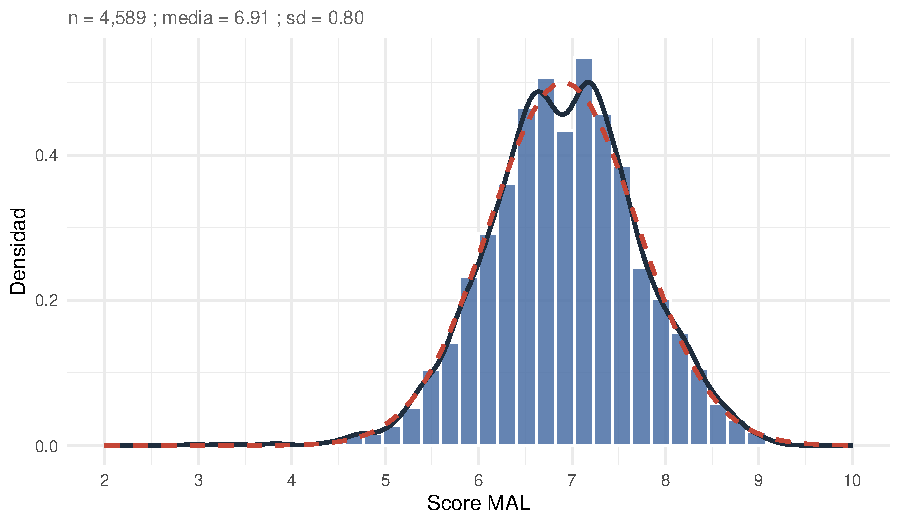
\includegraphics[keepaspectratio]{propuesta_files/figure-pdf/fig-score-dist-1.pdf}}

}

\caption{\label{fig-score-dist}Distribución del Score promedio en el
subconjunto de estudio. La línea continua corresponde a la densidad
estimada; la línea discontinua, a una densidad normal con la misma media
y desviación estándar.}

\end{figure}%

La distribución del Score (Figura 1) es notablemente simétrica, con
media 6.91 y desviación estándar 0.8. El soporte empírico se concentra
entre 4.5 y 8.5, lejos de los límites teóricos del rango {[}0, 10{]}, y
la densidad estimada se aproxima estrechamente a una normal de mismos
parámetros. Este hallazgo es relevante para el modelado: dado que el
Score reportado por MyAnimeList es ya un promedio sobre miles o millones
de calificaciones individuales, su distribución agregada cumple
aproximadamente las condiciones del Teorema Central del Límite, lo que
sugiere que una verosimilitud normal es razonable para la Pregunta 1,
sin necesidad de transformaciones de límites.

\begin{figure}[H]

\centering{

\pandocbounded{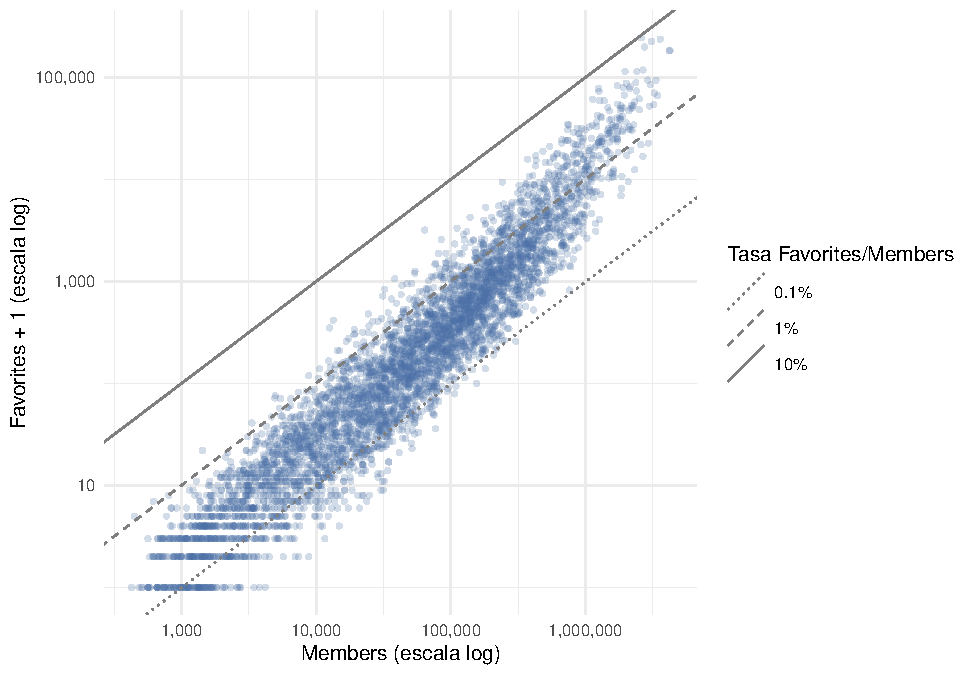
\includegraphics[keepaspectratio]{propuesta_files/figure-pdf/fig-members-favs-1.pdf}}

}

\caption{\label{fig-members-favs}Relación entre tamaño de la audiencia
(Members) y número de favoritos absolutos (Favorites + 1, escala log10).
Las líneas grises de referencia corresponden a tasas constantes de
favoritos del 0.1\%, 1\% y 10\%.}

\end{figure}%

La Figura 2 ilustra simultáneamente tres hechos centrales para la
Pregunta 2. Primero, ambas variables presentan extrema heterogeneidad:
Members varía desde decenas hasta varios millones (cuatro órdenes de
magnitud), justificando el uso de escala logarítmica. Segundo, la nube
de puntos se distribuye predominantemente entre las líneas de referencia
del 0.1\% y 1\%, confirmando que la tasa típica de fidelización es de
orden \(10^{-3}\) a \(10^{-2}\) --- y que esta tasa varía
sustancialmente entre obras. Tercero, la nube no se ajusta a una recta
única: existe dispersión vertical considerable a cualquier nivel de
Members, lo que constituye evidencia visual de la sobredispersión que
motiva el uso de un modelo Beta-Binomial en lugar de un modelo binomial
estándar.

\begin{figure}[H]

\centering{

\pandocbounded{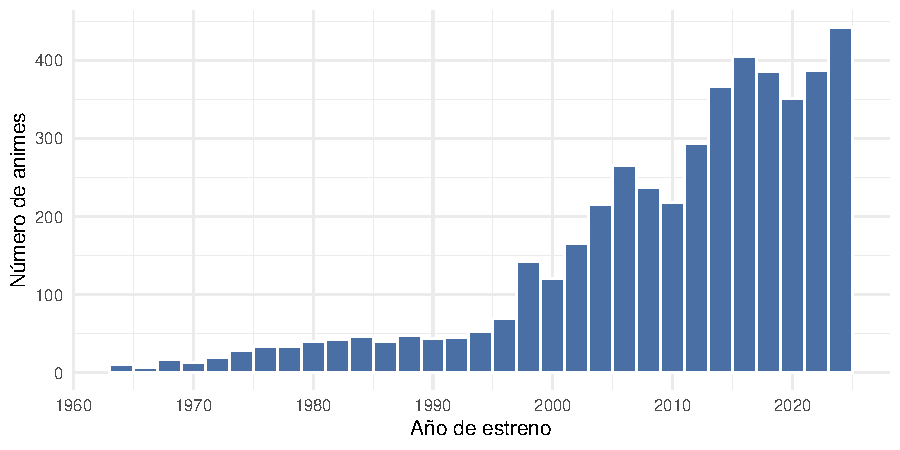
\includegraphics[keepaspectratio]{propuesta_files/figure-pdf/fig-cobertura-temporal-1.pdf}}

}

\caption{\label{fig-cobertura-temporal}Distribución temporal del
subconjunto de estudio por año de estreno.}

\end{figure}%

El subconjunto cubre obras estrenadas desde la década de 1960 hasta
2025, con una clara aceleración productiva a partir de los años 2000 que
refleja el crecimiento global de la industria. Esta amplitud temporal
introduce una potencial fuente de confusión en la Pregunta 2: animes
recientes han tenido menos tiempo para acumular tanto Members como
Favorites, y la dinámica de acumulación de cada métrica no es
necesariamente proporcional. La Sección 4.3 explorará si existe un
efecto sistemático del año sobre la tasa de favoritos.

\subsection{Lado de la producción: estudios y material
original}\label{lado-de-la-producciuxf3n-estudios-y-material-original}

\begin{figure}[H]

\centering{

\pandocbounded{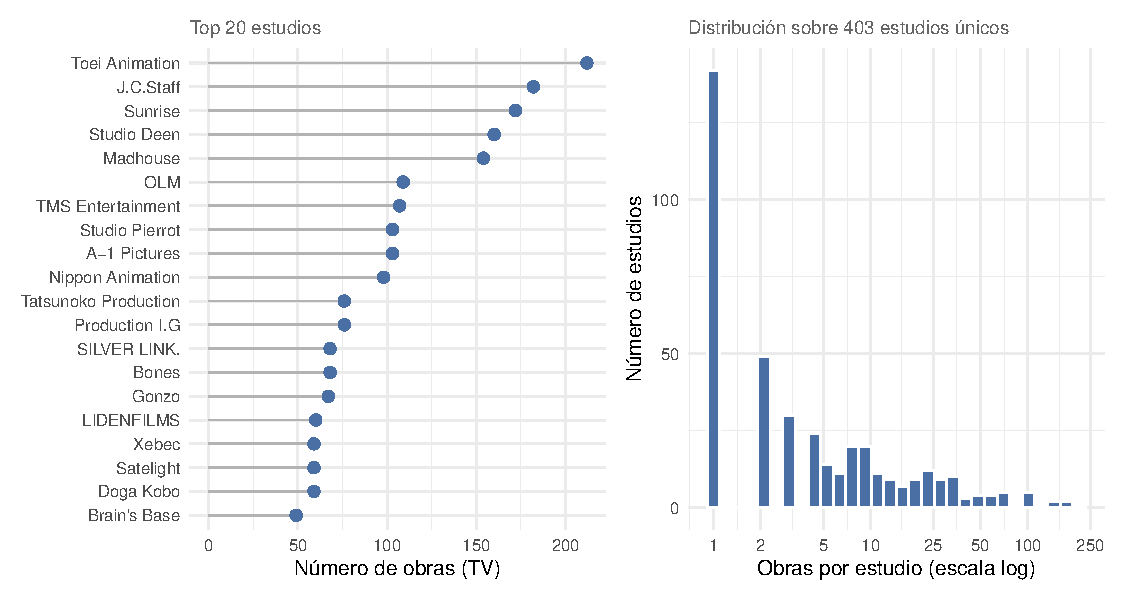
\includegraphics[keepaspectratio]{propuesta_files/figure-pdf/fig-studios-distribution-1.pdf}}

}

\caption{\label{fig-studios-distribution}Distribución del número de
obras por estudio en el subconjunto de estudio. Panel izquierdo: top 20
estudios. Panel derecho: histograma del número de obras por estudio en
escala log10.}

\end{figure}%

La Figura 4 revela la marcada heterogeneidad en la productividad de los
estudios. El panel izquierdo muestra que un puñado de estudios (Toei
Animation, J.C.Staff, Sunrise) concentra varios cientos de obras cada
uno, mientras que el panel derecho ---en escala logarítmica--- evidencia
que la distribución agregada es fuertemente asimétrica: la mediana de
obras por estudio es de unas pocas unidades, y una proporción
considerable de estudios tiene apenas una o dos producciones. Esta
heterogeneidad extrema constituye el argumento central a favor de un
enfoque jerárquico bayesiano: una estimación frecuentista por estudio
asignaría la misma confianza a una media basada en 200 obras que a una
media basada en 2, ignorando la diferencia drástica de información
disponible. El mecanismo de \emph{partial pooling} del modelo jerárquico
aborda precisamente este problema, encogiendo las estimaciones de
estudios poco informativos hacia el promedio global y preservando la
individualidad de los estudios con evidencia abundante.

\begin{figure}[H]

\centering{

\pandocbounded{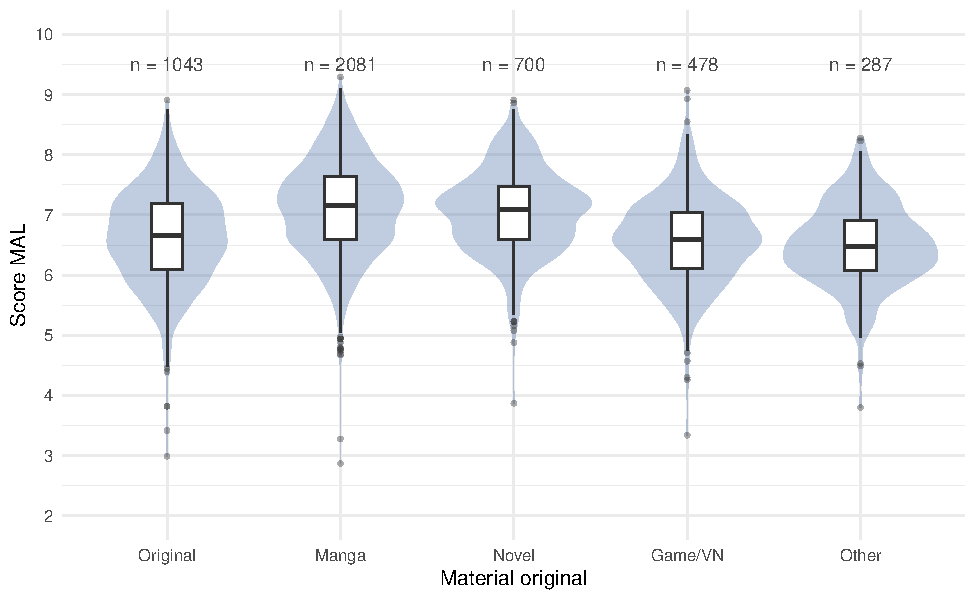
\includegraphics[keepaspectratio]{propuesta_files/figure-pdf/fig-score-by-source-1.pdf}}

}

\caption{\label{fig-score-by-source}Distribución del Score según el
material original adaptado. Las anotaciones indican el tamaño de muestra
de cada categoría.}

\end{figure}%

La Figura 5 sugiere que el material original adaptado guarda una
asociación moderada con el Score. Las adaptaciones de Manga y Novelas
(ligeras y convencionales) presentan medianas ligeramente superiores a
las obras Originales, mientras que las adaptaciones de Juegos / Visual
Novels muestran mayor variabilidad y una mediana algo más baja. Las
diferencias entre categorías son visibles pero no dramáticas, lo que es
consistente con la hipótesis de que el material original aporta
información parcial al pronóstico de calidad ---pero no determinante---;
el resto de la variabilidad en Score puede atribuirse a otros factores,
entre ellos el estudio responsable, lo que motiva incluir ambas
variables en el modelo.

\begin{figure}[H]

\centering{

\pandocbounded{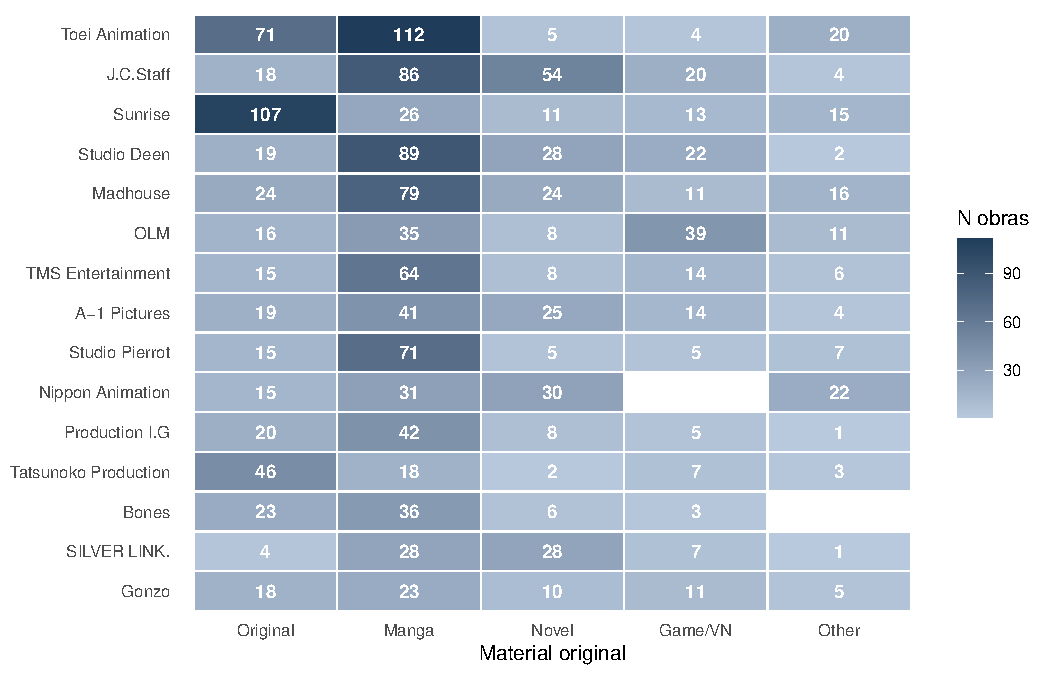
\includegraphics[keepaspectratio]{propuesta_files/figure-pdf/fig-studio-source-heatmap-1.pdf}}

}

\caption{\label{fig-studio-source-heatmap}Frecuencia de obras por
combinación Estudio × Material original (top 15 estudios). Las celdas
vacías corresponden a combinaciones sin observaciones.}

\end{figure}%

La Figura 6 cuantifica la dispersión empírica del cruce Estudio ×
Material original sobre los 15 estudios más productivos. La estructura
revela patrones claros: algunos estudios muestran una clara orientación
hacia un tipo de material ---Sunrise y Tatsunoko Production producen
mayoritariamente obras Originales, mientras que Toei Animation,
J.C.Staff y Studio Pierrot se inclinan fuertemente hacia adaptaciones de
Manga---; otros como Madhouse o Studio Deen muestran un portafolio más
diversificado a lo largo de varias categorías. Igualmente importante es
la abundancia de celdas con frecuencia muy baja, particularmente en las
categorías Novel y Game/VN: muchas combinaciones Estudio × Source están
escasamente representadas (varias con menos de 5 obras), e incluso
aparecen combinaciones sin observaciones, lo que reafirma la dificultad
de obtener estimaciones puntuales confiables para cada celda y refuerza
el caso para un modelo que combine información a través de la estructura
jerárquica.

\begin{figure}[H]

\centering{

\pandocbounded{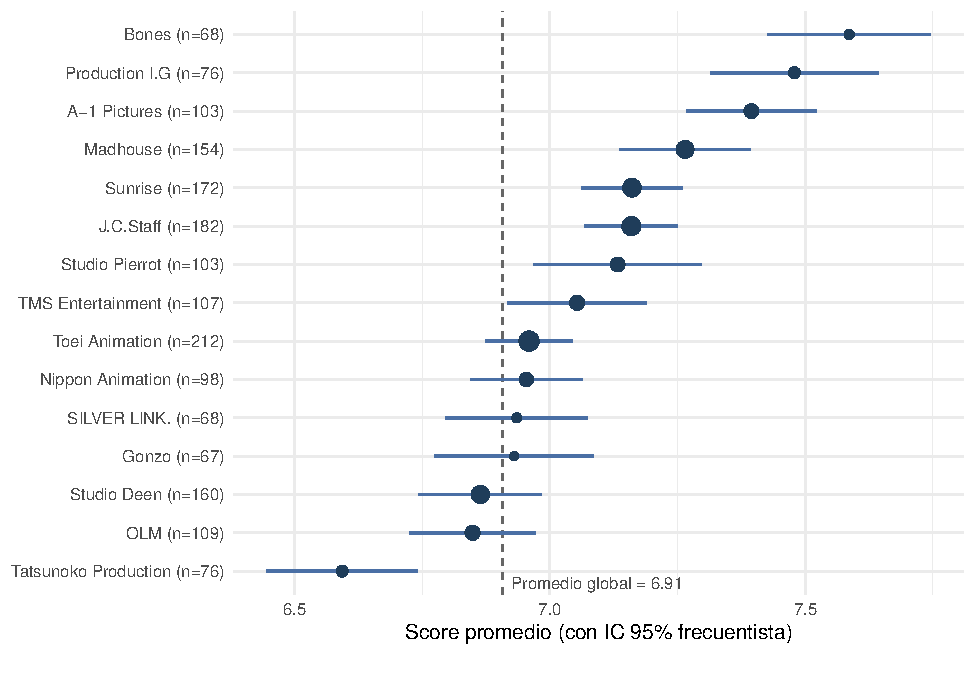
\includegraphics[keepaspectratio]{propuesta_files/figure-pdf/fig-studio-score-ci-1.pdf}}

}

\caption{\label{fig-studio-score-ci}Score promedio por estudio (top 15
por número de obras), con intervalo de confianza frecuentista al 95\%
basado en el error estándar de la media. La línea vertical discontinua
marca el promedio global. El número entre paréntesis indica el tamaño de
muestra.}

\end{figure}%

La Figura 7 sintetiza el problema central que motiva el enfoque
bayesiano. Cada punto representa la media muestral del Score para uno de
los 15 estudios más productivos; las barras horizontales son intervalos
de confianza frecuentistas al 95\% calculados sobre el error estándar de
la media. Tres observaciones se destacan. \textbf{Primero}, las medias
muestrales se distribuyen entre aproximadamente 6.59 y 7.59, sugiriendo
diferencias sistemáticas entre estudios: varios estudios presentan
intervalos de confianza que \textbf{no incluyen el promedio global}
(línea discontinua), tanto por encima (Bones, Production I.G, A-1
Pictures, Madhouse, J.C.Staff, Sunrise) como por debajo (Tatsunoko
Production), lo que indica diferencias estadísticamente detectables en
estos casos. \textbf{Segundo}, los intervalos de confianza varían
notablemente en amplitud: estudios con mayor número de obras (Toei
Animation con n=212, Sunrise con n=172) presentan intervalos estrechos,
mientras que estudios con menos obras tienen intervalos
considerablemente más anchos ---lo que refleja correctamente la
diferencia de información disponible, pero también sugiere que estudios
intermedios (n entre 60 y 100) podrían beneficiarse de un mecanismo de
combinación parcial de información. \textbf{Tercero}, esta figura está
restringida a los 15 estudios con mayor número de obras; al considerar
el conjunto completo de los 403 estudios presentes en la muestra ---de
los cuales más de 200 tienen menos de 5 obras--- la inestabilidad de las
estimaciones frecuentistas se vuelve aún más severa, situación que el
\emph{partial pooling} del modelo jerárquico bayesiano está
específicamente diseñado para manejar.

\subsection{Lado del consumo: géneros y
fidelización}\label{lado-del-consumo-guxe9neros-y-fidelizaciuxf3n}

\begin{longtable}[]{@{}lr@{}}
\caption{Distribución de la tasa de favoritos (Favorites/Members) en el
subconjunto de la Pregunta 2.}\tabularnewline
\toprule\noalign{}
Estadística & Valor \\
\midrule\noalign{}
\endfirsthead
\toprule\noalign{}
Estadística & Valor \\
\midrule\noalign{}
\endhead
\bottomrule\noalign{}
\endlastfoot
Mínimo & 0.000 \% \\
Percentil 25 & 0.182 \% \\
Mediana & 0.340 \% \\
Media & 0.522 \% \\
Percentil 75 & 0.603 \% \\
Percentil 90 & 1.105 \% \\
Percentil 99 & 3.149 \% \\
Máximo & 9.430 \% \\
Animes con tasa = 0 & 59 \\
Animes con tasa \textgreater{} 1\% & 520 \\
Animes con tasa \textgreater{} 5\% & 8 \\
\end{longtable}

La Tabla 3 cuantifica con precisión la forma de la distribución de la
tasa de fidelización. Tres rasgos son determinantes para el modelado.
Primero, la tasa típica es muy baja: la mediana se sitúa en torno al
0.34\%, y el 75\% de los animes tiene una tasa inferior al 0.6\%.
Segundo, la distribución presenta una cola derecha pronunciada: el
percentil 99 es aproximadamente diez veces la mediana, y el máximo
observado supera el 9\%. Tercero, una fracción no despreciable de animes
presenta tasa exactamente cero, y muchas tasas se encuentran muy cerca
de cero, lo que invalida un modelo binomial estándar (que asignaría a
estas observaciones probabilidades excesivamente bajas) y motiva el uso
de un modelo Beta-Binomial capaz de absorber la sobredispersión inducida
por estos extremos.

\begin{figure}[H]

\centering{

\pandocbounded{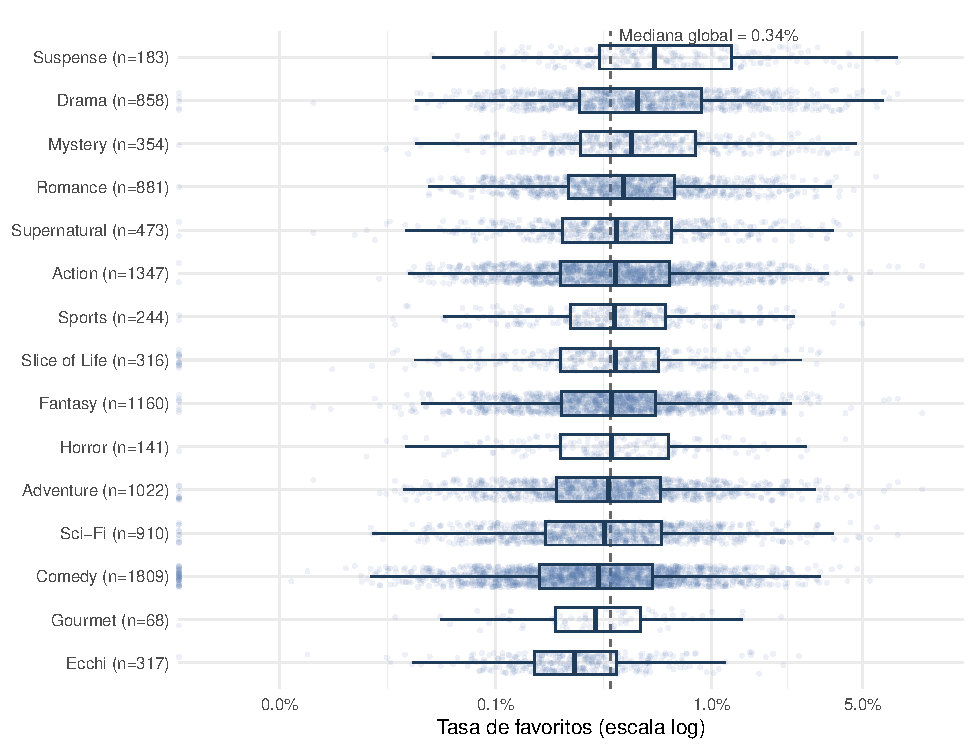
\includegraphics[keepaspectratio]{propuesta_files/figure-pdf/fig-fav-by-genre-1.pdf}}

}

\caption{\label{fig-fav-by-genre}Distribución de la tasa de favoritos
(Favorites/Members) por género, para los 15 géneros más frecuentes. Los
puntos individuales corresponden a animes; las cajas resumen la
distribución por género. Los géneros están ordenados por mediana
descendente. La línea vertical discontinua marca la mediana global.}

\end{figure}%

La Figura 8 revela que existen diferencias sustanciales y sistemáticas
entre géneros en términos de fidelización. Géneros como Suspense,
Mystery, Drama y Sci-Fi tienden a presentar medianas claramente
superiores a la mediana global, mientras que géneros más asociados al
consumo masivo o casual---como Comedy, Gourmet o Ecchi--- tienden a
generar tasas de favoritos sustancialmente más bajas. Una observación
particularmente interesante es la convivencia, dentro de cada género, de
una amplia dispersión: incluso géneros con mediana baja contienen animes
con tasas de fidelización extraordinariamente altas (varias veces la
mediana), evidenciando que el género impone una distribución de
probabilidad sobre la fidelización, no un valor determinístico. Esta
estructura es precisamente la que justifica un modelo de regresión
bayesiano sobre la tasa de favoritos: estimar el efecto medio del género
sobre el log-odds de la fidelización, controlando simultáneamente por
otras fuentes de variación. Asimismo, dado que un mismo anime suele
tener varias etiquetas de género simultáneamente (Action + Adventure +
Fantasy es una combinación común), las observaciones individuales
aparecen replicadas en distintos géneros en esta figura; en el modelo,
esta multiplicidad se manejará mediante variables indicadoras
simultáneas y priors débilmente informativos que regularizan los efectos
de géneros correlacionados.

\begin{figure}[H]

\centering{

\pandocbounded{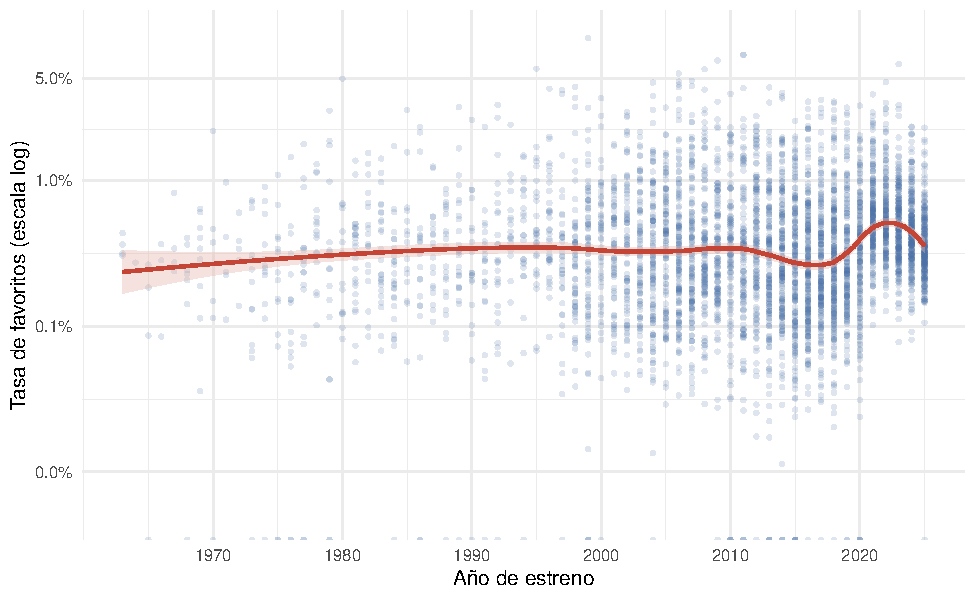
\includegraphics[keepaspectratio]{propuesta_files/figure-pdf/fig-fav-vs-year-1.pdf}}

}

\caption{\label{fig-fav-vs-year}Tasa de favoritos en función del año de
estreno. Cada punto representa un anime; la línea suavizada (LOESS)
resume la tendencia central. La caída pronunciada en años recientes
refleja un efecto de acumulación temporal, no necesariamente una caída
en la calidad del contenido.}

\end{figure}%

La Figura 9 ofrece un hallazgo descriptivo inesperado y relevante para
el modelado. Contrariamente a la hipótesis inicial de que los animes
recientes presentarían tasas de favoritos sistemáticamente más bajas
debido a un efecto de acumulación temporal ---dado que la métrica
Favorites debería tardar más en consolidarse que Members---, la curva
suavizada (LOESS) muestra una tendencia central notablemente plana a lo
largo de cinco décadas, con la mediana oscilando en un rango estrecho en
torno al 0.3 \%--0.4 \%. Una posible explicación es que el filtro
Members \(\geq\) 1000 aplicado a este subconjunto excluye animes
demasiado recientes para haber consolidado su audiencia, mitigando así
por construcción el sesgo temporal. Otra explicación complementaria es
que tanto Members como Favorites podrían seguir dinámicas de acumulación
de velocidades comparables, dado que añadir un anime a la lista de
seguimiento típicamente requiere haberlo visto al menos parcialmente.

Este hallazgo no implica que el año de estreno deba excluirse del
modelo; por el contrario, justifica incluirlo como variable de control
para descartar formalmente efectos temporales más sutiles ---por
ejemplo, posibles interacciones género × año asociadas al auge de
ciertos subgéneros (como Isekai dentro de Fantasy en años recientes) o
cambios en las normas de calificación de la comunidad MAL. La
incorporación del año como covariable funcionará entonces como una
salvaguarda metodológica: si el efecto resulta marginal en la inferencia
bayesiana, se podrá reportar con tranquilidad; si surge una interacción
no visible en la marginal, el modelo la capturará.

\subsection{Comparación cruzada: ¿calidad y fidelización son la misma
cosa?}\label{comparaciuxf3n-cruzada-calidad-y-fidelizaciuxf3n-son-la-misma-cosa}

\begin{figure}[H]

\centering{

\pandocbounded{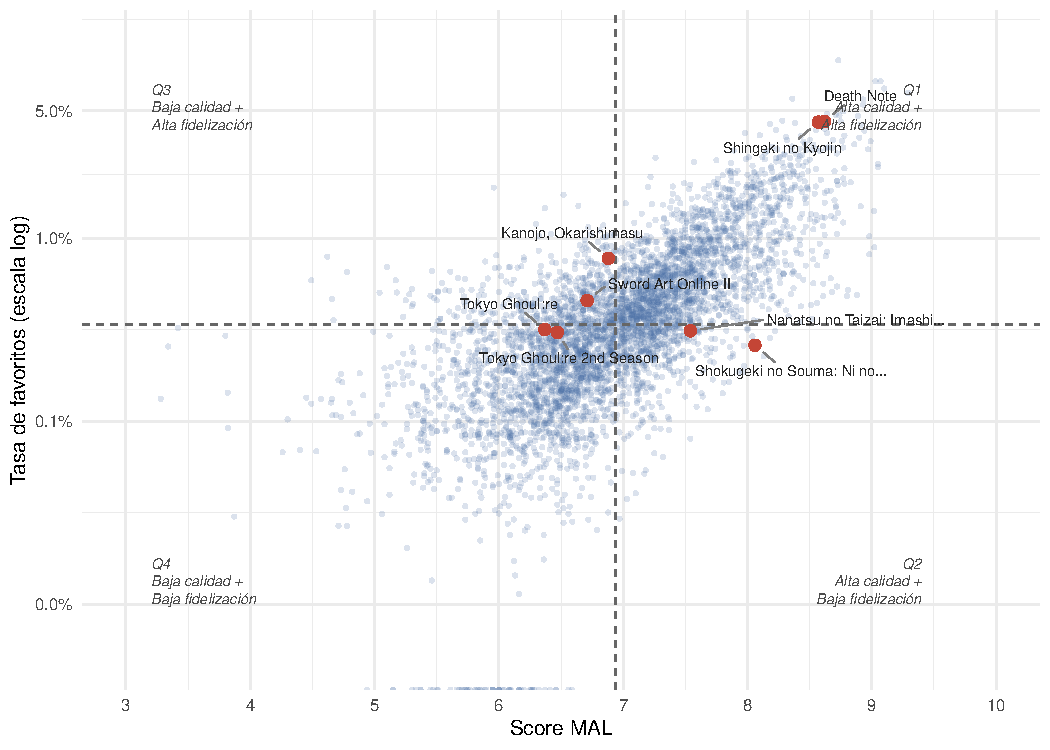
\includegraphics[keepaspectratio]{propuesta_files/figure-pdf/fig-score-vs-favrate-1.pdf}}

}

\caption{\label{fig-score-vs-favrate}Relación entre Score MAL (eje x) y
tasa de favoritos (eje y, escala log) para cada anime del subconjunto de
la Pregunta 2. Las líneas discontinuas marcan las medianas globales y
definen cuatro cuadrantes. Los puntos rojos identifican animes
representativos seleccionados por su popularidad (Members) dentro de
cada cuadrante.}

\end{figure}%

La Figura 10 condensa la pregunta central que motiva el diseño dual de
este proyecto: ¿son la calidad evaluada (Score) y la fidelización
profunda (tasa Favorites/Members) dos dimensiones distintas del éxito de
un anime, o constituyen esencialmente la misma información expresada en
escalas diferentes? La respuesta empírica es matizada. La correlación de
Pearson entre el Score y log₁₀(tasa de favoritos) es 0.60, y la
correlación de Spearman alcanza 0.73, indicando una asociación positiva
moderada-alta y monótona pero claramente alejada de la unidad. En otras
palabras: los animes mejor evaluados tienden, en promedio, a generar
mayor fidelización profunda, pero una porción sustancial de la
variabilidad de cada métrica es independiente de la otra. Esto descarta
la posibilidad de que las dos preguntas de investigación sean
redundantes.

La distribución de los animes en los cuatro cuadrantes formados por las
medianas globales (Score = 6.94, tasa de favoritos = 0.34 \%) confirma
cuantitativamente esta conclusión. Los cuadrantes ``concordantes'' Q1
(alta calidad y alta fidelización) y Q4 (baja calidad y baja
fidelización) concentran aproximadamente el 78 \% de la muestra,
reflejando la correlación positiva subyacente. Sin embargo, el 22 \%
restante ---distribuido casi simétricamente entre Q2 (alta calidad pero
baja fidelización) y Q3 (baja calidad pero alta fidelización)---
constituye un conjunto sustancial de obras (cerca de 1.000 animes) donde
las dos dimensiones divergen abiertamente. Es precisamente en este 22 \%
donde las inferencias de las preguntas 1 y 2 producirían rankings
sustancialmente distintos, y donde el valor del enfoque dual se
manifiesta con mayor claridad.

Los animes destacados en rojo ---seleccionados como los más populares de
cada cuadrante--- ilustran de forma concreta los perfiles industriales
subyacentes. En Q1 aparecen títulos como Shingeki no Kyojin (Attack on
Titan) y Death Note, obras consagradas en el imaginario global del
anime, donde excelencia evaluativa y devoción del público se refuerzan
mutuamente. Q2 muestra un patrón observacional sugerente: ambos
representantes ---Shokugeki no Souma: Ni no Sara y Nanatsu no Taizai:
Imashime no Fukkatsu--- son secuelas, lo que podría indicar que las
temporadas posteriores heredan grandes audiencias del éxito de la
primera entrega pero raramente concentran sobre sí mismas el
comportamiento de marcar como ``favorita'' ---patrón digno de
exploración complementaria. Q3, por su parte, contiene obras como Sword
Art Online II y Kanojo, Okarishimasu, que combinan una calificación
moderada con una tasa de favoritos elevada ---perfil compatible con
audiencias polarizadas pero con núcleos de seguidores intensamente
comprometidos. Finalmente, Q4 incluye casos como las temporadas
posteriores de Tokyo Ghoul:re, donde tanto la calificación promedio como
la tasa de favoritos se sitúan por debajo de las medianas globales,
reflejando obras que no logran consolidar ni excelencia evaluativa ni
adhesión afectiva.

Esta tipología empírica sustenta el diseño metodológico del proyecto. Si
las dos métricas estuvieran fuertemente correlacionadas (por ejemplo, r
\textgreater{} 0.9), formular dos preguntas de investigación distintas
constituiría redundancia analítica: los modelos producirían
esencialmente el mismo ordenamiento de estudios y géneros, solo que en
escalas diferentes. La asociación moderada observada (r = 0.60)
garantiza, en cambio, que cada pregunta capte un aspecto genuinamente
distinto del fenómeno: la Pregunta 1 identifica qué configuraciones
productivas (estudio × material original) tienden a generar obras
evaluadas como de alta calidad por la comunidad amplia, mientras que la
Pregunta 2 identifica qué contenidos (géneros) generan vínculos
afectivos profundos entre los espectadores que sí los consumen. En la
sección de discusión del informe final, los resultados de ambos modelos
se contrastarán explícitamente para identificar configuraciones donde un
estudio o un género destaque en una dimensión pero no en la otra ---lo
que constituirá una de las contribuciones interpretativas centrales del
proyecto.

\section{Próximos pasos}\label{pruxf3ximos-pasos}

A partir de las observaciones empíricas presentadas en el análisis
descriptivo, el desarrollo del informe final se estructurará en torno a
la implementación, validación e interpretación de los modelos bayesianos
correspondientes a cada una de las dos preguntas de investigación.

Para la Pregunta 1, planeamos especificar un modelo jerárquico bayesiano
de regresión sobre el Score, con verosimilitud normal ---justificada por
la aproximación a la normalidad observada en la Figura 1--- y efectos
por estudio, incluyendo el material original (Source) como covariable de
interés. La estructura jerárquica implementará partial pooling sobre los
efectos por estudio, abordando directamente la heterogeneidad muestral
documentada en las Figuras 4 y 7. Variables como el número de episodios
o el año de estreno podrán incorporarse como covariables adicionales
para mejorar la calidad de la inferencia, sujeto a su contribución
empírica.

Para la Pregunta 2, planeamos especificar un modelo de regresión
bayesiana sobre la proporción Favorites/Members con una verosimilitud
capaz de manejar la sobredispersión ---justificada por la dispersión
vertical observada en la Figura 2 y por la presencia de tasas
extremadamente bajas o nulas documentada en la Tabla 3---, efectos por
género codificados como variables indicadoras múltiples, y controles por
año de estreno y por el tamaño de la audiencia. Priors débilmente
informativos sobre los efectos de género operarán como mecanismo de
regularización ante la correlación esperable entre etiquetas
frecuentemente co-ocurrentes.

En ambos casos, el proceso analítico incorporará: chequeos predictivos
previos para validar la razonabilidad de la estructura del modelo antes
de la inferencia; diagnósticos estándar de convergencia de las cadenas
MCMC (\(\hat{R}\), número efectivo de muestras, transiciones
divergentes); chequeos predictivos posteriores para evaluar el ajuste
del modelo a los datos; análisis de sensibilidad respecto a la elección
de priors ---siguiendo las prácticas estándar del flujo de trabajo
bayesiano descritas por Gelman et~al. (2013) y McElreath (2020); e
interpretación de los resultados mediante intervalos creíbles y
distribuciones posteriores de cantidades de interés. Adicionalmente, en
la sección de discusión del informe final se realizará un contraste
explícito entre los hallazgos de los dos modelos, identificando
configuraciones (estudios y géneros) donde la calidad evaluativa y la
fidelización profunda divergen ---en línea con la tipología empírica
documentada en la Sección 4.4.

\section*{Referencias}\label{referencias}
\addcontentsline{toc}{section}{Referencias}

\phantomsection\label{refs}
\begin{CSLReferences}{1}{0}
\bibitem[\citeproctext]{ref-apriansyah2025mal}
Apriansyah, Syahrul. 2025. {«{MyAnimeList 2025}: Comprehensive {A}nime
{D}ataset»}. Conjunto de datos en línea; Kaggle.
\url{https://www.kaggle.com/datasets/syahrulapriansyah2/myanimelist-2025}.

\bibitem[\citeproctext]{ref-aja2025report}
Association of Japanese Animations (AJA). 2024-\/-2025. {«Anime Industry
Report»}. Reportes anuales sobre la industria de la animación japonesa.
\url{https://aja.gr.jp/english/japan-anime-data}.

\bibitem[\citeproctext]{ref-gelman2013bayesian}
Gelman, Andrew, John B. Carlin, Hal S. Stern, David B. Dunson, Aki
Vehtari, y Donald B. Rubin. 2013. \emph{Bayesian Data Analysis}. 3rd ed.
Boca Raton, FL: Chapman \& Hall/CRC.

\bibitem[\citeproctext]{ref-mcelreath2020rethinking}
McElreath, Richard. 2020. \emph{Statistical Rethinking: A {B}ayesian
Course with Examples in {R} and {S}tan}. 2nd ed. Boca Raton, FL: Chapman
\& Hall/CRC.

\bibitem[\citeproctext]{ref-mal2025}
MyAnimeList LLC. 2025. {«{MyAnimeList}: Base de datos y comunidad de
anime y manga»}. \url{https://myanimelist.net}.

\end{CSLReferences}




\end{document}
